\subsection{Use Case 2: Get Diagnosis}

 \subsubsection{General Description}
\begin{tabular}{|p{.2\linewidth}|p{.65\linewidth}|}
\hline 
ID: & Get Diagnosis \\ \hline
Goal: & The user gets the diagnosis for their individual complains \\ \hline
Precondition: &  The user entered their symptoms via text or scanned their skin via our skin scanning feature\\ \hline
Postcondition: & The user gets their diagnosis \\ \hline
Involved Users: & User: Someone who uses our app \\ \hline
\end{tabular}

\subsubsection{UI}

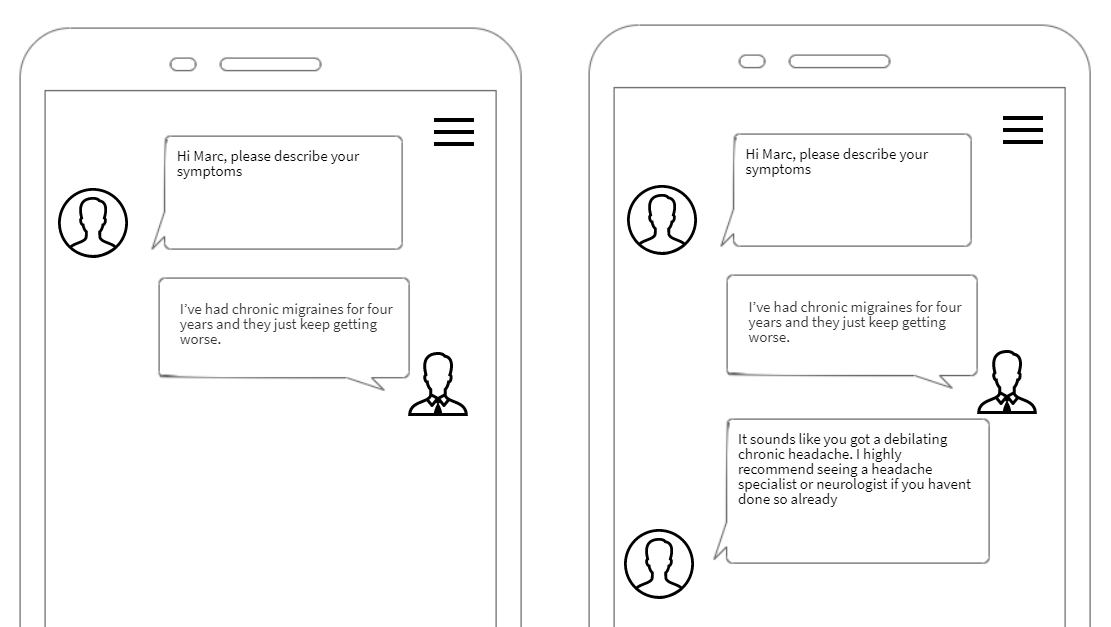
\includegraphics[scale=1.2]{SystemSpec/Usecases/Mocks/getdiagnosis01.PNG}\\
The user receives their diagnosis in form of an chat message from DoctorRobert after they entered their symptoms. If the answer contains any complicated medical terms, DoctorRobert will simplify it and provide further reading material regarding the complicated terms.

\subsubsection{The Standard Use}
\begin{figure}[H]
\centering
    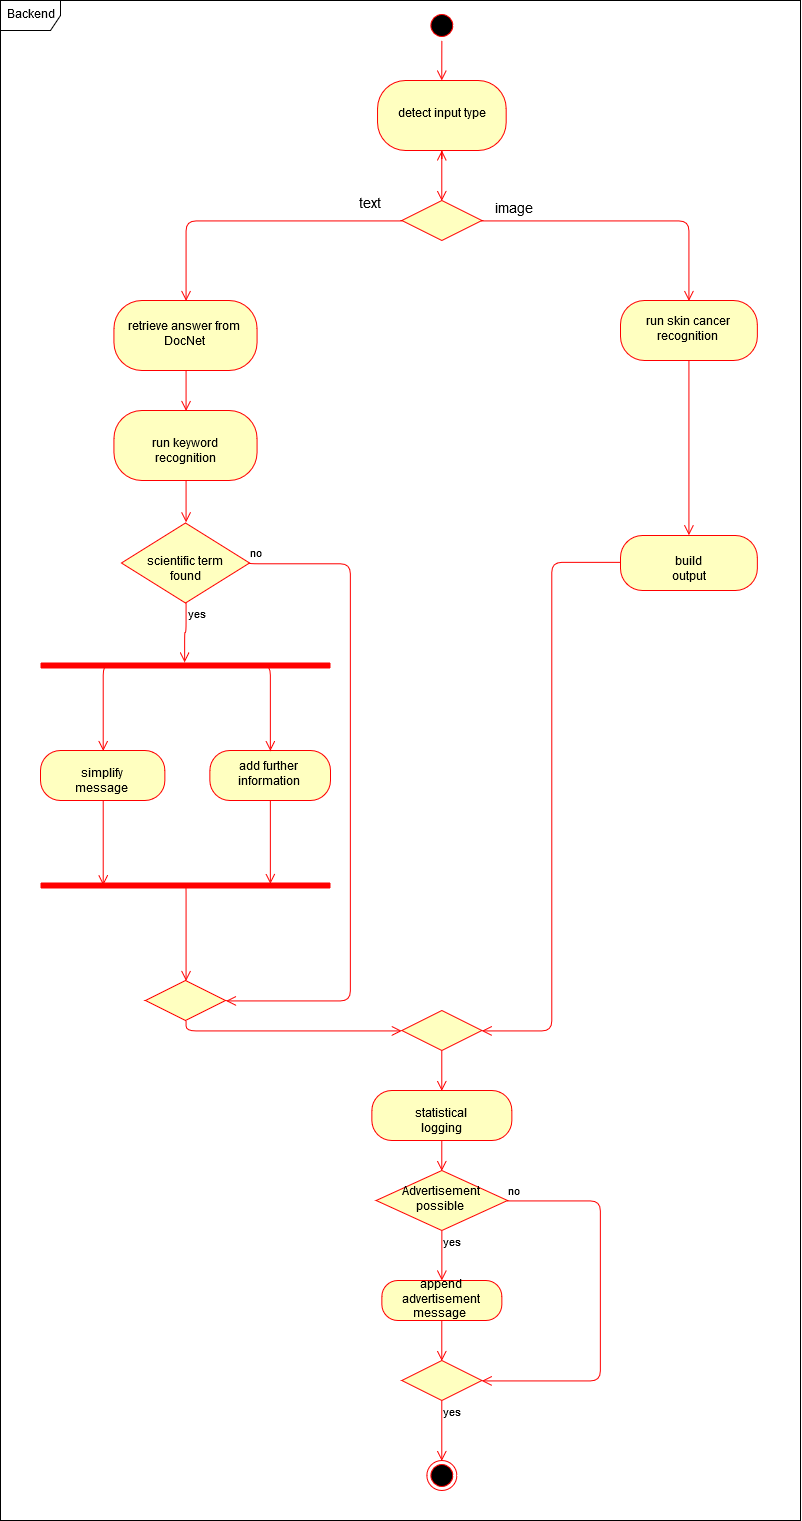
\includegraphics[scale=0.32]{SystemSpec/Usecases/Diagrams/GetDiagnosisActivity.png}
\caption{\label{fig:blue_rectangle}get diagnosis activity}
\end{figure}

\paragraph{detect input type}
Our back-end will determine whether the input is entered in the form of a text or as a picture.

\paragraph{retrieve answer from DocNet}
The input will run trough our AI algorithm and an response will be generated.

\paragraph{run keyword recognition}
The generated response from activity "retrieve answer from DocNet" will be checked for certain keywords.

\paragraph{scientific term found}
If the keyword recognition finds terms which are too scientific or hard to understand, the two use cases "simplify message" and "add further information" will be triggered. 

\paragraph{simplify message}
Based on the keyword recognition an algorithm tries to simplify and make the final response more readable.

\paragraph{add further information}
Based on the keyword recognition certain keywords will receive explanations so a user can understand them. This will be realised by hyperlinking further reading material to the word.

\paragraph{run skin cancer recognition}
If the input is a picture it will run through our computer vision AI. The AI will determine a percentage of how confident it is that the user has skin cancer. This result will be used to create an diagnosis message in "build output".

\paragraph{build output}

A answer will be assembled based on the output of the previous activity.

\paragraph{anonymous logging of data for our advertisement feature}
Before the back-end will send and terminate the message to provide anonymity. We will include relevant data from the answer to the users question in our statistics. This process will only capture data that can not be pin pointed to a specific user. The statistics are used for consumer analysis and marketing purposes.

\paragraph{append advertisement message}

If the final answer to the query(image or text) contains any keywords that match the description of an paying advertiser, an corresponding ad will be shown. \hypertarget{AdIllustration}{An illustration is shown below.}
\begin{center}
    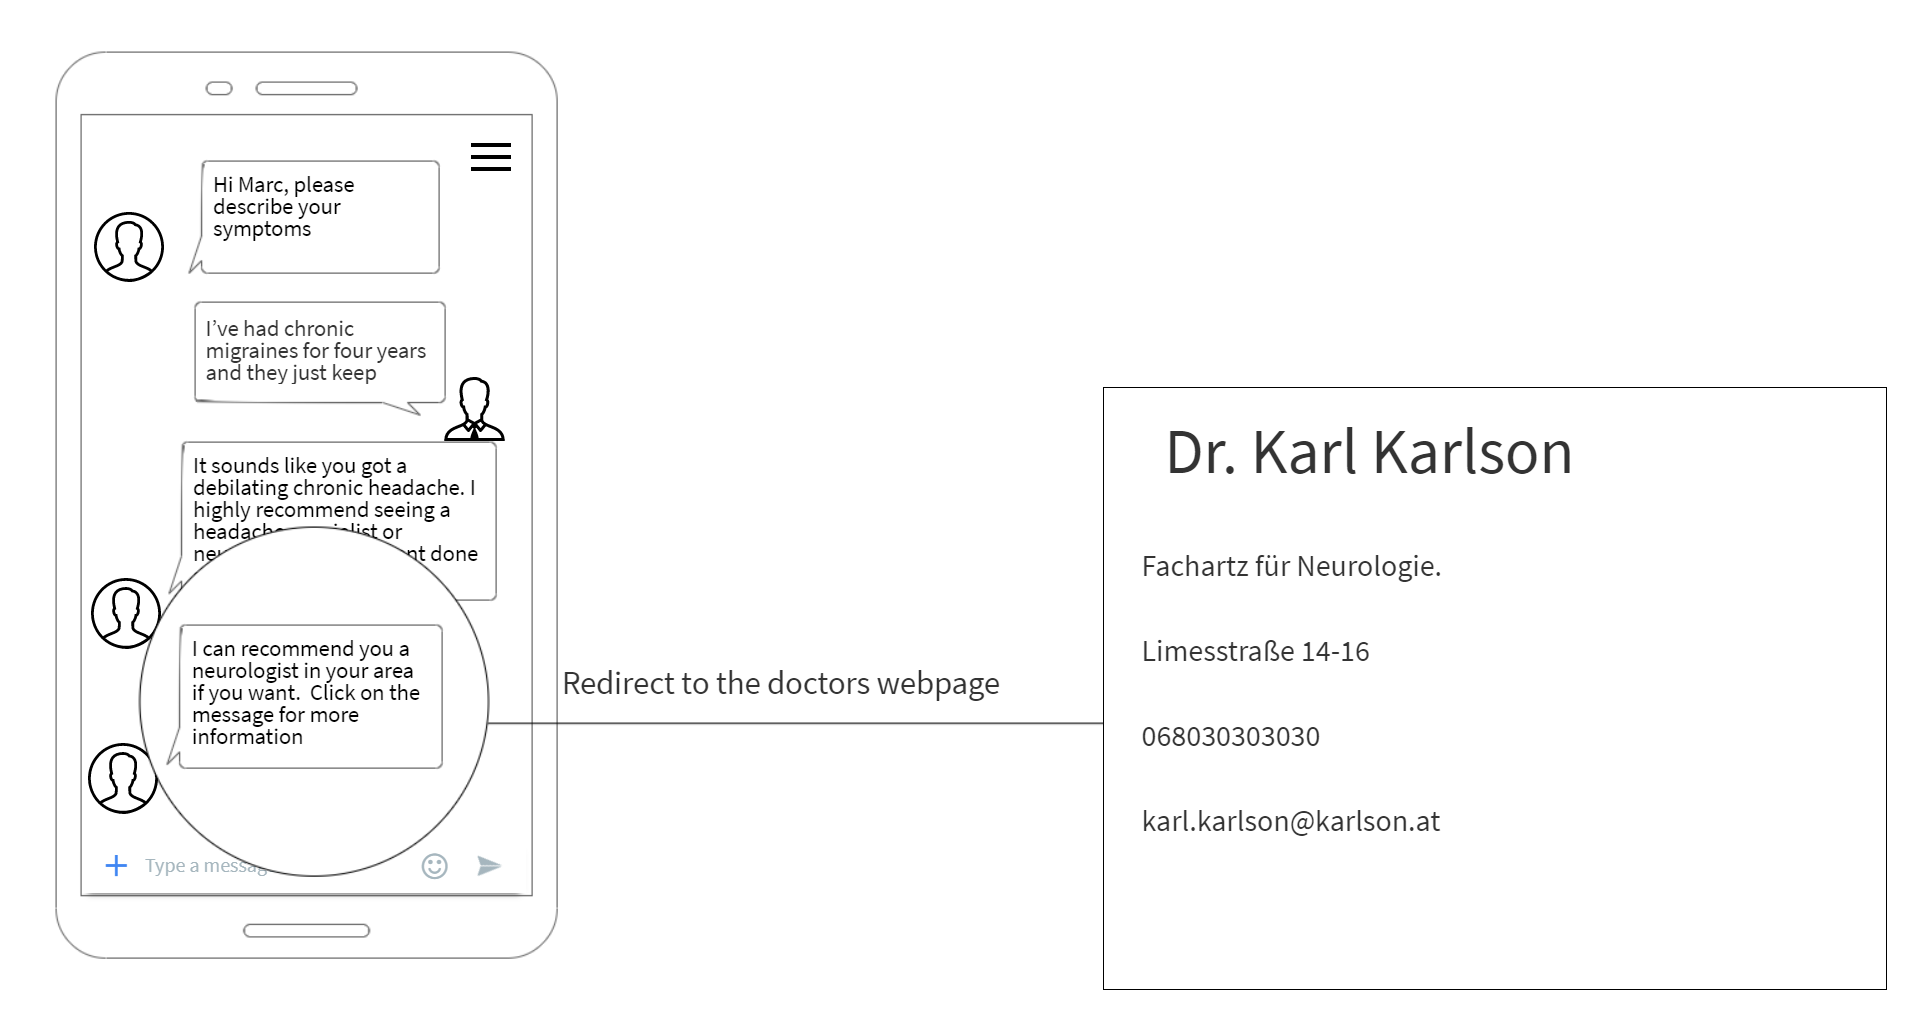
\includegraphics[scale=0.8]{SystemSpec/Usecases/Mocks/advertismentMock.PNG}
\end{center}

\subsubsection{The Non-Standard Use}

\begin{itemize}
    \item User enters something that doesn't make sense
    
    If a user enters nonsensical symptoms or no real  symptoms at all our system will not be able to recognize the fault therefor the input will be treated as normal and the user will receive an equally rubbish answer as their input. 
    
    \item \hypertarget{ScanSkinNonStandard}{The user submits a picture of something other than skin.}
        
        \begin{center}
            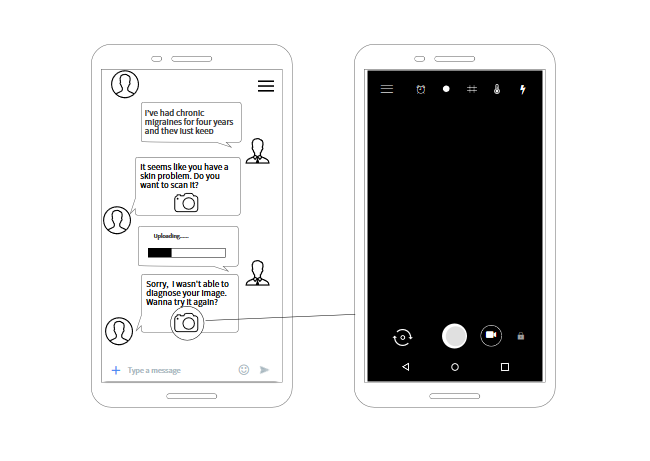
\includegraphics[scale=.7]{SystemSpec/Usecases/Mocks/getdiagnosis02.png}\\
        \end{center}{}
    
        If the percentage of confidence in the diagnosis of our scanning algorithm is too low, like for example when a user submits a faulty image, the user will be asked to take another picture instead of getting an diagnosis like shown above.
    
    \item AI misprediction

    Sometimes the AI is not able to interpret the given query the right way. Unfortunately, we are not able to detect extreme mispredictions yet. In order to avoid the users distrust, measure to clarify this imperfection have to be set. For instance, showing the user a reminder about mentioned imperfections at the start of the application. 

\end{itemize}

\pagebreak
